\documentclass{standalone}
\usepackage{tikz}
\usepackage{pgfplots}
\usepackage{tikz-3dplot}
\tdplotsetmaincoords{60}{115}
\pgfplotsset{compat=newest}

\usepackage{scalefnt}

 
\begin{document}

{\scalefont{0.3}
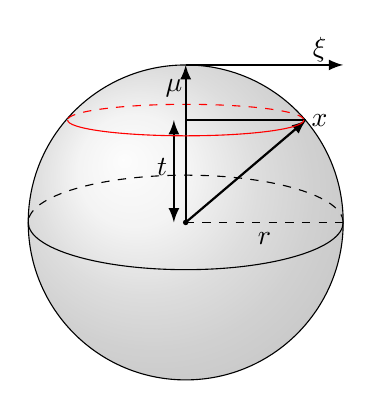
\begin{tikzpicture}
	
	% Ball
	\shade[ball color = gray!40, opacity = 0.3] (0,0) circle (2cm);
  
  	% Outline of sphere
  	\draw (0,0) circle (2cm);

  	 % Draw back arc swept out by the component perpendicular to mu   
  	\draw[red,dashed] (1.5,1.3) arc  (0:180:1.5 and 0.2) ; 
  
  	% Front equator line 	
 	\draw (-2,0) arc (180:360:2 and 0.6);
 	
  	% Back equator line 
 	\draw[dashed] (2,0) arc (0:180:2 and 0.6);
 	
 	% Circle at origin
  	\fill[fill=black] (0,0) circle (1pt);
  	
  	% Radius
 	\draw[dashed] (0,0) -- node[below]{$r$} (2,0);

	% Axes
  	\draw[thick,solid,-latex] (0,0) -- (0,2);
  	\draw[thick,solid,-latex] (0,2) -- (2,2);
  
  	% t
  	\draw[thick,solid,latex-latex] (-.15,0) -- (-.15,1.3);
  	\node at (-0.3,.7) {$t$};
  
  	% component perp to mu
  	\draw[thick,solid] (0,1.3) -- (1.53,1.3);
  	%\node at (.5,1.5) {$\sqrt{1-t^{2}}$};
  
  	% xi
  	\draw[thick,solid,-latex] (0,0) -- (1.53,1.3);
  	\node at (1.7,2.2) {$\xi$};
  	
  	% X
  	\node at (1.7,1.3) {$x$};
  
 	% mu axis
  	\node at (-0.15,1.7) {$\mu$};  
  
  	% xi axis
  	  
  
 	% Draw front arc swept out by the component perpendicular to mu   
 	\draw[red] (-1.5,1.3) arc  (180:360:1.5 and 0.2) ;  
  
\end{tikzpicture}
}
 
\end{document}